\documentclass[11pt,a4paper]{article}

\usepackage[utf8]{inputenc}
\usepackage[spanish,es-tabla]{babel}
\usepackage[margin=2.3cm]{geometry}
\usepackage{amsmath,amsfonts,amssymb}
\usepackage{graphicx}
\usepackage{booktabs}
\usepackage{tabularx}
\usepackage{array}
\usepackage{xcolor}
\usepackage{hyperref}
\usepackage{microtype}
\usepackage{caption}
\usepackage{float}
\usepackage{fancyhdr}
\usepackage{titlesec}
\usepackage{enumitem}

\definecolor{primary}{RGB}{15, 23, 42}
\definecolor{accent}{RGB}{5, 150, 105}
\definecolor{secondary}{RGB}{30, 58, 138}
\definecolor{coral}{RGB}{220, 38, 38}

\hypersetup{
    colorlinks=true,
    linkcolor=secondary,
    citecolor=accent,
    urlcolor=secondary
}

\pagestyle{fancy}
\fancyhf{}
\rhead{\textcolor{gray}{\small Grupo 02 | Estimación de Gastos de Seguros Médicos}}
\lhead{\textcolor{gray}{\small Sistemas Inteligentes y Machine Learning}}
\cfoot{\thepage}

\titleformat{\section}{\large\bfseries\color{primary}}{\thesection.}{0.5em}{}[\titlerule]
\titleformat{\subsection}{\normalsize\bfseries\color{secondary}}{\thesubsection.}{0.5em}{}

\begin{document}

\begin{titlepage}
    \centering
    \vspace*{1.5cm}
    {\Huge\bfseries\color{primary} UNIVERSIDAD NACIONAL DE INGENIERÍA\par}
    \vspace{0.4cm}
    {\Large\color{secondary} Facultad de Ingeniería / Departamento de Computación e Informática\par}
    \vspace{0.2cm}
    {\large Curso: Sistemas Inteligentes y Machine Learning (2026-II)\par}
    
    \vspace{2.5cm}
    \rule{\linewidth}{1.5pt}\par
    \vspace{0.5cm}
    {\LARGE\bfseries\color{primary} ESTIMACIÓN DE GASTOS DE SEGUROS MÉDICOS INDIVIDUALES MEDIANTE MODELOS SUPERVISADOS DE REGRESIÓN SIN FUGA DE INFORMACIÓN\par}
    \vspace{0.3cm}
    {\large\itshape Informe Académico y Técnico de Investigación Aplicada (Grupo 02)\par}
    \vspace{0.5cm}
    \rule{\linewidth}{1.5pt}\par
    
    \vspace{3cm}
    \begin{minipage}{0.48\textwidth}
        \begin{flushleft} \large
            \textbf{Integrantes:}\\
            Venegas Calizaya, Gerardo Matías\\
            Equipo de Proyecto -- Grupo 02\\
            \textit{Data \& ML Engineering}
        \end{flushleft}
    \end{minipage}
    \begin{minipage}{0.48\textwidth}
        \begin{flushright} \large
            \textbf{Docente:}\\
            Mg. / Dr. Docente Titular\\
            \textit{Cátedra de Machine Learning}\\
            \vspace{0.5cm}
            \textbf{Fecha de Entrega:}\\
            1 de Noviembre de 2026
        \end{flushright}
    \end{minipage}
    
    \vfill
    {\small Lima, Perú}
\end{titlepage}

\begin{abstract}
El presente trabajo desarrolla y evalúa un sistema predictivo supervisado de regresión para estimar los cargos médicos anuales individuales (\texttt{charges}) a partir del conjunto de datos \textit{Medical Cost Personal Datasets} ($n = 1,338$), disponible en Kaggle. La problemática central aborda la incertidumbre financiera en la suscripción y cálculo de reservas técnicas para aseguradoras de salud en el instante inicial de contratación ($t = 0$). Se diseñó un protocolo metodológico estricto para mitigar el riesgo de fuga de información (\textit{data leakage}): se efectuó una partición inicial 80/20 con semilla fija (\texttt{random\_state = 42}), aislando un conjunto de prueba reservado ($n = 268$) evaluado una única vez al final del estudio. Dentro de una arquitectura de \texttt{Pipeline} y \texttt{ColumnTransformer}, se aplicó imputación robusta (\texttt{SimpleImputer}), escalado estándar (\texttt{StandardScaler}) y codificación \textit{One-Hot} (\texttt{OneHotEncoder}) ajustados exclusivamente sobre los pliegues de entrenamiento. Se compararon tres familias algorítmicas obligatorias (\texttt{LinearRegression}, \texttt{KNeighborsRegressor} y \texttt{SVR}) frente a una línea base ingenua (\texttt{DummyRegressor}). Mediante Validación Cruzada de 5 folds idénticos y optimización de hiperparámetros con \texttt{GridSearchCV}, el modelo \texttt{SVR (Optimizado)} con núcleo RBF ($C = 10,000$, $\gamma = \text{'scale'}$, $\epsilon = 1.0$) resultó ganador previo a la inspección de prueba con un $\text{MAE}_{\text{CV}} = \$2,014.67 \pm \$322.28$ y $R^2 = 0.8289$. En la prueba final reservada, el modelo ganador alcanzó un $\text{MAE} = \$1,803.44$ USD (reducción del $81.20\%$ respecto a la línea base de $\$9,593.34$), $\text{RMSE} = \$4,832.09$ y $R^2 = 0.8496$. El análisis específico del Grupo 02 evidenció que, si bien el error nominal es mayor en fumadores ($\text{MAE} = \$4,119.27$) que en no fumadores ($\text{MAE} = \$1,219.08$) debido a la escala monetaria media ($\$33,204.10$ vs. $\$7,862.09$), el error relativo es inferior en fumadores ($12.41\%$ vs. $15.51\%$) y el $R^2$ intra-grupo alcanza $0.6778$. Se enfatiza explícitamente que estas estimaciones corresponden a asociaciones observacionales y no a relaciones de causalidad médica directa. El sistema se desplegó en una aplicación interactiva en Streamlit.
\par\vspace{0.3cm}
\noindent\textbf{Palabras clave:} Aprendizaje supervisado, Regresión, Soporte de Vectores para Regresión (SVR), Prevención de Data Leakage, Validación Cruzada, Streamlit.
\end{abstract}

\newpage
\tableofcontents
\newpage

\section{Introducción y Planteamiento del Problema}

\subsection{Contexto y Relevancia Actuarial}
En la industria aseguradora de salud y la administración de planes colectivos de medicina prepagada, uno de los desafíos operacionales y financieros más críticos consiste en anticipar con exactitud y objetividad el costo esperado por siniestralidad de cada asegurado. La fijación inadecuada de primas conduce a dos escenarios desfavorables:
\begin{enumerate}[leftmargin=*]
    \item \textbf{Déficit de suscripción y riesgo de solvencia:} Si la prima calculada subestima los gastos reales en pólizas de alta siniestralidad, la aseguradora incurre en insuficiencia de reservas técnicas.
    \item \textbf{Selección adversa y pérdida de mercado:} Si las tarifas sobreestiman arbitrariamente el riesgo de los perfiles saludables, dichos usuarios migran hacia la competencia, concentrando una cartera con mayor siniestralidad relativa.
\end{enumerate}
Tradicionalmente, las instituciones han empleado tablas actuariales estáticas basadas en segmentaciones unidimensionales. Sin embargo, estas aproximaciones no logran capturar complejas interacciones no lineales entre hábitos de vida, biomarcadores metabólicos y factores demográficos.

\subsection{Pregunta Predictiva Central}
La presente investigación responde a la siguiente interrogante operativa:
\begin{quote}
    \textit{¿Con qué precisión cuantitativa (medida en error absoluto medio en dólares estadounidenses, MAE) es posible estimar los costos médicos individuales anuales de un asegurado en el momento exacto de suscripción ($t = 0$), empleando algoritmos supervisados de regresión entrenados bajo un diseño libre de fuga de datos?}
\end{quote}

\subsection{Usuario Decisor, Momento de Uso y Decisión Respaldada}
\begin{itemize}[leftmargin=*]
    \item \textbf{Usuario Decisor:} El sistema está dirigido al analista actuarial, al suscriptor técnico de pólizas (\textit{medical underwriter}) y a los comités de gestión integral de riesgos de aseguradoras de salud.
    \item \textbf{Momento de Inferencia ($t = 0$):} El modelo interviene de manera sincrónica al momento en que un individuo solicita una nueva afiliación o en la tarificación de renovaciones anuales, \textbf{antes} de que ocurran los siniestros del período de cobertura.
    \item \textbf{Decisión que respalda:} Estimación objetiva de la prima pura de riesgo, asignación de reservas de siniestros no ocurridos e identificación de perfiles para incorporación temprana a programas de medicina preventiva.
\end{itemize}

\subsection{Esquema Conceptual de Entrada y Salida}
El flujo funcional modela la relación matemática:
\begin{equation}
    \hat{y} = f(\mathbf{X})
\end{equation}
donde el vector de entrada está constituido por 6 variables observables antes del inicio de la póliza:
\begin{equation}
    \mathbf{X} = [\text{age}, \text{bmi}, \text{children}, \text{sex}, \text{smoker}, \text{region}]
\end{equation}
y la salida predicha es el costo médico acumulado anual facturado en dólares estadounidenses: $\hat{y} \in \mathbb{R}^+$ (USD \$).

\section{Objetivos y Criterios de Éxito}

\subsection{Objetivo General}
Desarrollar, validar y desplegar en una aplicación web interactiva (Streamlit) un sistema predictivo supervisado para estimar los cargos médicos anuales individuales (\texttt{charges}) en el conjunto \textit{Medical Cost Personal Datasets}, comparando bajo un protocolo experimental de 5 folds idénticos tres modelos supervisados obligatorios (\texttt{LinearRegression}, \texttt{KNeighborsRegressor} y \texttt{SVR}) frente a una línea base (\texttt{DummyRegressor}), garantizando ausencia absoluta de fuga de información y logrando en un conjunto de prueba reservado (20\%) un $\text{MAE} < \$3,500$ USD y un coeficiente de determinación $R^2 \ge 0.75$.

\subsection{Objetivos Específicos}
\begin{enumerate}[leftmargin=*]
    \item \textbf{OE1 (Diagnóstico de Calidad y Exploración):} Identificar la calidad del conjunto de datos (valores nulos, duplicados y tipología) y analizar la asimetría y dispersión de la variable monetaria \texttt{charges}, evaluando su relación bivariada con la edad, índice de masa corporal y consumo de tabaco.
    \item \textbf{OE2 (Arquitectura de Preprocesamiento sin Fuga):} Diseñar e implementar un esquema modular con \texttt{ColumnTransformer} que impute, escale y codifique las ramas numéricas y categóricas nominales exclusivamente dentro de pipelines ajustados sobre datos de entrenamiento.
    \item \textbf{OE3 (Entrenamiento y Optimización Cruzada):} Evaluar mediante Validación Cruzada de 5 folds idénticos el rendimiento de los modelos candidatos y optimizar los hiperparámetros de KNN y SVR mediante \texttt{GridSearchCV} usando MAE como métrica rectora.
    \item \textbf{OE4 (Evaluación Reservada e Inferencia Desplegada):} Evaluar una sola vez en el 20\% de prueba el modelo ganador seleccionado antes del test, analizar los errores por niveles de gasto y hábito tabáquico aclarando la ausencia de causalidad directa, y desplegar el pipeline en \texttt{app.py} para inferencia interactiva.
\end{enumerate}

\subsection{Criterios de Aceptación Cuantitativos y Costo de los Errores}
El criterio de éxito se fijó ex-ante:
\begin{itemize}[leftmargin=*]
    \item \textbf{Métrica Primaria:} $\text{MAE} < \$3,500$ USD (menor es mejor), superando holgadamente a la línea base ingenua.
    \item \textbf{Métricas Secundarias:} $R^2 \ge 0.75$ y minimización de la brecha entre MAE y RMSE.
    \item \textbf{Costo Asimétrico del Error:} La subestimación ($\hat{y} < y$) genera insuficiencia de reservas técnicas y riesgo de solvencia institucional, mientras que la sobreestimación ($\hat{y} > y$) provoca pérdida de competitividad comercial y selección adversa.
\end{itemize}

\section{Metodología y Procedencia de los Datos}

\subsection{Procedencia, Licencia y Ficha Técnica}
El conjunto analizado corresponde al \textit{Medical Cost Personal Datasets}, publicado por Miri Choi en Kaggle, originado a partir de los datos actuariales recopilados en el texto clásico \textit{Machine Learning with R} de Brett Lantz.
\begin{itemize}[leftmargin=*]
    \item \textbf{Identificador y URL:} \url{https://www.kaggle.com/datasets/mirichoi0218/insurance}
    \item \textbf{Archivo analizado:} \texttt{insurance.csv} (Versión 1)
    \item \textbf{Licencia:} Database Contents License (DbCL) v1.0.
    \item \textbf{Dimensiones:} $1,338$ filas $\times$ $7$ columnas.
    \item \textbf{Integridad:} 0 valores nulos en la totalidad de celdas; 1 fila duplicada exacta detectada (índices 195 y 581: asegurado de 19 años, hombre, BMI 30.59, 0 hijos, no fumador, noroeste). Se conservó por ser un perfil demográfico perfectamente plausible en una población real.
\end{itemize}

\subsection{Partición Experimental Anti-Fuga (Etapa 6)}
Para asegurar que las transformaciones numéricas y categóricas no extraigan parámetros del conjunto de validación o prueba, la partición se ejecutó en primer orden:
\begin{itemize}[leftmargin=*]
    \item \textbf{Tasa de partición:} $80\%$ entrenamiento ($n = 1,070$) y $20\%$ prueba reservada ($n = 268$).
    \item \textbf{Configuración:} \texttt{train\_test\_split(test\_size=0.20, random\_state=42, shuffle=True)}.
    \item \textbf{Verificación:} Intersección de índices entre entrenamiento y prueba estrictamente igual a 0 registros compartidos.
\end{itemize}

\subsection{Tratamiento y Transformación con \texttt{ColumnTransformer} (Etapa 7)}
El preprocesamiento se desacopló en dos ramas independientes:
\begin{enumerate}[leftmargin=*]
    \item \textbf{Rama Numérica (\texttt{age}, \texttt{bmi}, \texttt{children}):} Imputación mediante \texttt{SimpleImputer(strategy='median')} y estandarización mediante \texttt{StandardScaler()} ($\mu = 0$, $\sigma = 1$). El escalado es indispensable para evitar que variables en decenas monopolicen las distancias en KNN o los productos internos en SVR.
    \item \textbf{Rama Categórica Nominal (\texttt{sex}, \texttt{smoker}, \texttt{region}):} Imputación por moda mediante \texttt{SimpleImputer(strategy='most\_frequent')} y codificación \textit{One-Hot} mediante \texttt{OneHotEncoder(handle\_unknown='ignore', sparse\_output=False)}.
    \item \textbf{Variable Objetivo (\texttt{charges}):} Se mantiene intacta en su unidad monetaria original (\$ USD) sin transformación logarítmica para preservar la interpretabilidad financiera directa de los residuales actuariales.
\end{enumerate}

\subsection{Algoritmos Evaluados y Esquema de Validación}
Se implementaron 4 pipelines completos:
\begin{enumerate}[leftmargin=*]
    \item \textbf{DummyRegressor (Línea Base):} Predice la media de entrenamiento ($\hat{y} = \bar{y}_{\text{train}}$).
    \item \textbf{LinearRegression (OLS):} Modelo lineal aditivo paramétrico por mínimos cuadrados ordinarios.
    \item \textbf{KNeighborsRegressor (KNN):} Regresión no paramétrica basada en promedios ponderados de vecindarios locales.
    \item \textbf{SVR (Support Vector Regressor):} Regresión por vectores de soporte con función de pérdida $\epsilon$-insensible y núcleo de base radial (RBF).
\end{enumerate}
La validación cruzada consistió en \textbf{5 folds idénticos} (\texttt{KFold(n\_splits=5, shuffle=True, random\_state=42)}) ejecutados exclusivamente sobre las $1,070$ observaciones de entrenamiento.

\newpage
\section{Resultados y Evidencias Cuantitativas}

\subsection{Tablas Estándar del Proyecto (T1 a T9)}

\begin{table}[H]
\centering
\caption{\textbf{Tabla T1:} Diccionario de Variables y Análisis Anti-Fuga (Etapa 3)}
\footnotesize
\begin{tabularx}{\textwidth}{l p{3.2cm} l l l c l}
\toprule
\textbf{Variable} & \textbf{Definición Operacional} & \textbf{Tipo} & \textbf{Rol} & \textbf{Unidad / Categorías} & \textbf{Ex-Ante} & \textbf{Decisión} \\
\midrule
\texttt{age} & Edad biológica cumplida & int64 & Predictora ($X$) & Años (18 a 64) & Sí & Incluir \\
\texttt{sex} & Sexo biológico del titular & str & Predictora ($X$) & \texttt{female}, \texttt{male} & Sí & Incluir \\
\texttt{bmi} & Índice de masa corporal & float64 & Predictora ($X$) & $\text{kg/m}^2$ (15.96 a 53.13) & Sí & Incluir \\
\texttt{children} & Dependientes en la póliza & int64 & Predictora ($X$) & Conteo (0 a 5) & Sí & Incluir \\
\texttt{smoker} & Consumo habitual de tabaco & str & Predictora ($X$) & \texttt{yes}, \texttt{no} & Sí & Incluir \\
\texttt{region} & Ubicación geográfica & str & Predictora ($X$) & 4 regiones cardinales & Sí & Incluir \\
\texttt{charges} & Gastos médicos facturados & float64 & Objetivo ($y$) & USD (\$1,121 a \$63,770) & No & Excluir de $X$ \\
\bottomrule
\end{tabularx}
\end{table}

\begin{table}[H]
\centering
\caption{\textbf{Tabla T2:} Diagnóstico de Calidad de Datos (Etapa 5)}
\footnotesize
\begin{tabularx}{\textwidth}{l c c c p{4.2cm} p{4.8cm}}
\toprule
\textbf{Variable} & \textbf{Tipo} & \textbf{Nulos} & \textbf{Nulos (\%)} & \textbf{Valores Extremos (Criterio IQR)} & \textbf{Medida Adoptada} \\
\midrule
\texttt{age} & int64 & 0 & 0.00\% & 0 atípicos IQR (rango [18, 64]) & Conservar; StandardScaler en Pipeline. \\
\texttt{sex} & object & 0 & 0.00\% & 0 inválidos (female: 662, male: 676) & Conservar; OneHotEncoder en Pipeline. \\
\texttt{bmi} & float64 & 0 & 0.00\% & 9 extremos IQR ($0.67\%$) $> 47.29$ & Conservar; casos reales de obesidad mórbida. \\
\texttt{children} & int64 & 0 & 0.00\% & 0 atípicos IQR (rango [0, 5]) & Conservar; StandardScaler en Pipeline. \\
\texttt{smoker} & object & 0 & 0.00\% & 0 inválidos (no: 1064, yes: 274) & Conservar; OneHotEncoder en Pipeline. \\
\texttt{region} & object & 0 & 0.00\% & 0 inválidos (4 regiones) & Conservar; OneHotEncoder en Pipeline. \\
\texttt{charges} & float64 & 0 & 0.00\% & 139 extremos IQR ($10.39\%$) $> \$34,489$ & Conservar; 97.84\% son fumadores. Evaluar con MAE. \\
\bottomrule
\end{tabularx}
\end{table}

\begin{table}[H]
\centering
\caption{\textbf{Tabla T3:} Partición de Datos 80/20 (Etapa 6)}
\footnotesize
\begin{tabularx}{\textwidth}{l c c c c c c}
\toprule
\textbf{Subconjunto} & \textbf{Registros ($n$)} & \textbf{Proporción} & \textbf{Media `charges` (\$)} & \textbf{Mediana (\$)} & \textbf{Desv. Est. (\$)} & \textbf{Filas Compartidas} \\
\midrule
\textbf{Entrenamiento (Train)} & 1,070 & 80.00\% & \$13,346.09 & \$9,412.96 & \$12,078.38 & 0 \\
\textbf{Prueba Reservada (Test)} & 268 & 20.00\% & \$12,967.68 & \$9,193.84 & \$12,248.87 & 0 \\
\textbf{Total Dataset} & 1,338 & 100.00\% & \$13,270.42 & \$9,382.03 & \$12,110.01 & 0 \\
\bottomrule
\end{tabularx}
\end{table}

\begin{table}[H]
\centering
\caption{\textbf{Tabla T4:} Esquema de Preprocesamiento sin Fuga (Etapa 7)}
\footnotesize
\begin{tabularx}{\textwidth}{l p{3.5cm} p{3.2cm} p{3.2cm} p{4.5cm}}
\toprule
\textbf{Rama} & \textbf{Variables} & \textbf{Imputación} & \textbf{Codificación / Escala} & \textbf{Justificación Metodológica} \\
\midrule
\textbf{Numérica} & \texttt{age}, \texttt{bmi}, \texttt{children} & \texttt{SimpleImputer(median)} & \texttt{StandardScaler()} & Mediana tolera extremos en BMI. StandardScaler equipara varianzas para SVR y KNN. \\
\textbf{Categórica Binaria} & \texttt{sex}, \texttt{smoker} & \texttt{SimpleImputer(mode)} & \texttt{OneHotEncoder(ignore)} & Indicadores 0/1 sin imponer falso orden. \\
\textbf{Categórica Multiclase} & \texttt{region} & \texttt{SimpleImputer(mode)} & \texttt{OneHotEncoder(ignore)} & Evita distancias espurias entre regiones. \\
\textbf{Objetivo ($y$)} & \texttt{charges} & No aplica (0 nulos) & Escala original (\$ USD) & Preserva interpretabilidad monetaria directa. \\
\bottomrule
\end{tabularx}
\end{table}

\begin{table}[H]
\centering
\caption{\textbf{Tabla T5:} Comparación en Validación Cruzada 5-Fold en Entrenamiento (Etapa 10)}
\footnotesize
\begin{tabularx}{\textwidth}{l c c c c c c c c}
\toprule
\textbf{Modelo Pipeline} & \textbf{F1 MAE} & \textbf{F2 MAE} & \textbf{F3 MAE} & \textbf{F4 MAE} & \textbf{F5 MAE} & \textbf{Media MAE (\$)} & \textbf{DE MAE (\$)} & \textbf{Media $R^2$} \\
\midrule
\textbf{DummyRegressor (Baseline)} & 9,187 & 9,211 & 9,384 & 8,760 & 8,492 & \textbf{9,007.09} & 326.06 & -0.0042 \\
\textbf{LinearRegression} & 4,215 & 4,498 & 4,380 & 3,892 & 4,188 & \textbf{4,234.98} & 277.28 & 0.7389 \\
\textbf{KNN ($k=5$)} & 3,780 & 3,891 & 3,612 & 3,420 & 3,568 & \textbf{3,654.66} & 184.48 & 0.7543 \\
\textbf{SVR (Defecto, $C=1.0$)} & 8,450 & 8,560 & 8,610 & 8,012 & 7,731 & \textbf{8,272.97} & 350.26 & -0.0987 \\
\bottomrule
\end{tabularx}
\end{table}

\begin{table}[H]
\centering
\caption{\textbf{Tabla T6:} Optimización de Hiperparámetros con GridSearchCV (Etapa 11)}
\footnotesize
\begin{tabularx}{\textwidth}{l p{4.2cm} c p{4.2cm} c c c}
\toprule
\textbf{Modelo} & \textbf{Espacio de Búsqueda} & \textbf{Comb.} & \textbf{Mejor Configuración} & \textbf{CV Antes (\$)} & \textbf{CV Después (\$)} & \textbf{Mejora} \\
\midrule
\textbf{KNN} & $k \in [3..15]$, weights, $p \in [1,2]$ & 24 & $k=5$, distance, Manhattan ($p=1$) & \$3,654.66 & \textbf{\$3,274.14} & -10.41\% \\
\textbf{SVR} & kernel, $C \in [10^2..10^4]$, $\gamma$, $\epsilon$ & 72 & RBF, $C=10^4$, $\gamma=\text{'scale'}$, $\epsilon=1.0$ & \$8,272.97 & \textbf{\$2,014.67} & \textbf{-75.65\%} \\
\bottomrule
\end{tabularx}
\end{table}

\begin{table}[H]
\centering
\caption{\textbf{Tabla T7:} Decisión y Selección Razonada del Modelo Previa al Test (Etapa 12)}
\footnotesize
\begin{tabularx}{\textwidth}{l p{4.5cm} c c c c l}
\toprule
\textbf{Candidato} & \textbf{Configuración Final} & \textbf{MAE CV (\$)} & \textbf{DE MAE (\$)} & \textbf{RMSE CV (\$)} & \textbf{$R^2$ CV} & \textbf{Decisión} \\
\midrule
\textbf{DummyRegressor} & \texttt{strategy='mean'} & 9,007.09 & 326.06 & 12,017.19 & -0.0042 & Baseline de referencia \\
\textbf{LinearRegression} & Mínimos Cuadrados (OLS) & 4,234.98 & 277.28 & 6,123.35 & 0.7389 & Descartado (alto error aditivo) \\
\textbf{KNN Optimizado} & $k=5$, Distancia, Manhattan & 3,274.14 & 263.34 & 5,539.27 & 0.7860 & Descartado (segundo lugar) \\
\textbf{SVR Optimizado} & \textbf{RBF, $C=10^4$, $\gamma=\text{'scale'}$, $\epsilon=1$} & \textbf{2,014.67} & \textbf{322.28} & \textbf{4,941.56} & \textbf{0.8289} & \textbf{GANADOR BLOQUEADO} \\
\bottomrule
\end{tabularx}
\end{table}

\begin{table}[H]
\centering
\caption{\textbf{Tabla T8:} Prueba Final sobre el Conjunto Reservado (Etapa 13)}
\footnotesize
\begin{tabularx}{\textwidth}{l c c c c c}
\toprule
\textbf{Métrica en Test ($n=268$)} & \textbf{Unidad} & \textbf{SVR Optimizado} & \textbf{DummyRegressor} & \textbf{Mejora Absoluta} & \textbf{Mejora Relativa} \\
\midrule
\textbf{MAE (Métrica Primaria)} & USD (\$) & \textbf{\$1,803.44} & \$9,593.34 & \textbf{-\$7,789.89} & \textbf{-81.20\%} \\
\textbf{RMSE (Métrica Secundaria)} & USD (\$) & \textbf{\$4,832.09} & \$12,465.61 & \textbf{-\$7,633.52} & \textbf{-61.24\%} \\
\textbf{$R^2$ (Varianza Explicada)} & Proporción & \textbf{0.8496} & -0.0009 & \textbf{+0.8505} & \textbf{84.96\% explicada} \\
\bottomrule
\end{tabularx}
\end{table}

\begin{table}[H]
\centering
\caption{\textbf{Tabla T9:} Demostración de Predicciones Nuevas Plausibles (Etapa 15)}
\footnotesize
\begin{tabularx}{\textwidth}{l c c c c c c c p{4cm}}
\toprule
\textbf{Caso} & \textbf{Edad} & \textbf{Sexo} & \textbf{BMI} & \textbf{Hijos} & \textbf{Fuma} & \textbf{Región} & \textbf{Predicción ($\hat{y}$)} & \textbf{Explicación Actuarial} \\
\midrule
\textbf{Caso 1} & 22 & F & 21.8 & 0 & no & NW & \textbf{\$2,545.38} & Riesgo basal mínimo: normopeso y juventud. \\
\textbf{Caso 2} & 41 & M & 27.4 & 3 & no & NE & \textbf{\$8,049.71} & Costo medio: incremento regular por edad y 3 hijos. \\
\textbf{Caso 3} & 27 & F & 23.5 & 0 & yes & SW & \textbf{\$16,556.97} & Salto intermedio por tabaco activo sin obesidad. \\
\textbf{Caso 4} & 61 & F & 31.2 & 1 & no & SE & \textbf{\$13,632.43} & Gasto elevado por edad (61) sin salto de tabaco. \\
\textbf{Caso 5} & 52 & M & 36.8 & 2 & yes & SE & \textbf{\$47,134.61} & Sinergia crítica: edad $>50$, tabaco y obesidad severa. \\
\bottomrule
\end{tabularx}
\end{table}

\subsection{Evidencias Gráficas del Estudio}

\begin{figure}[H]
\centering
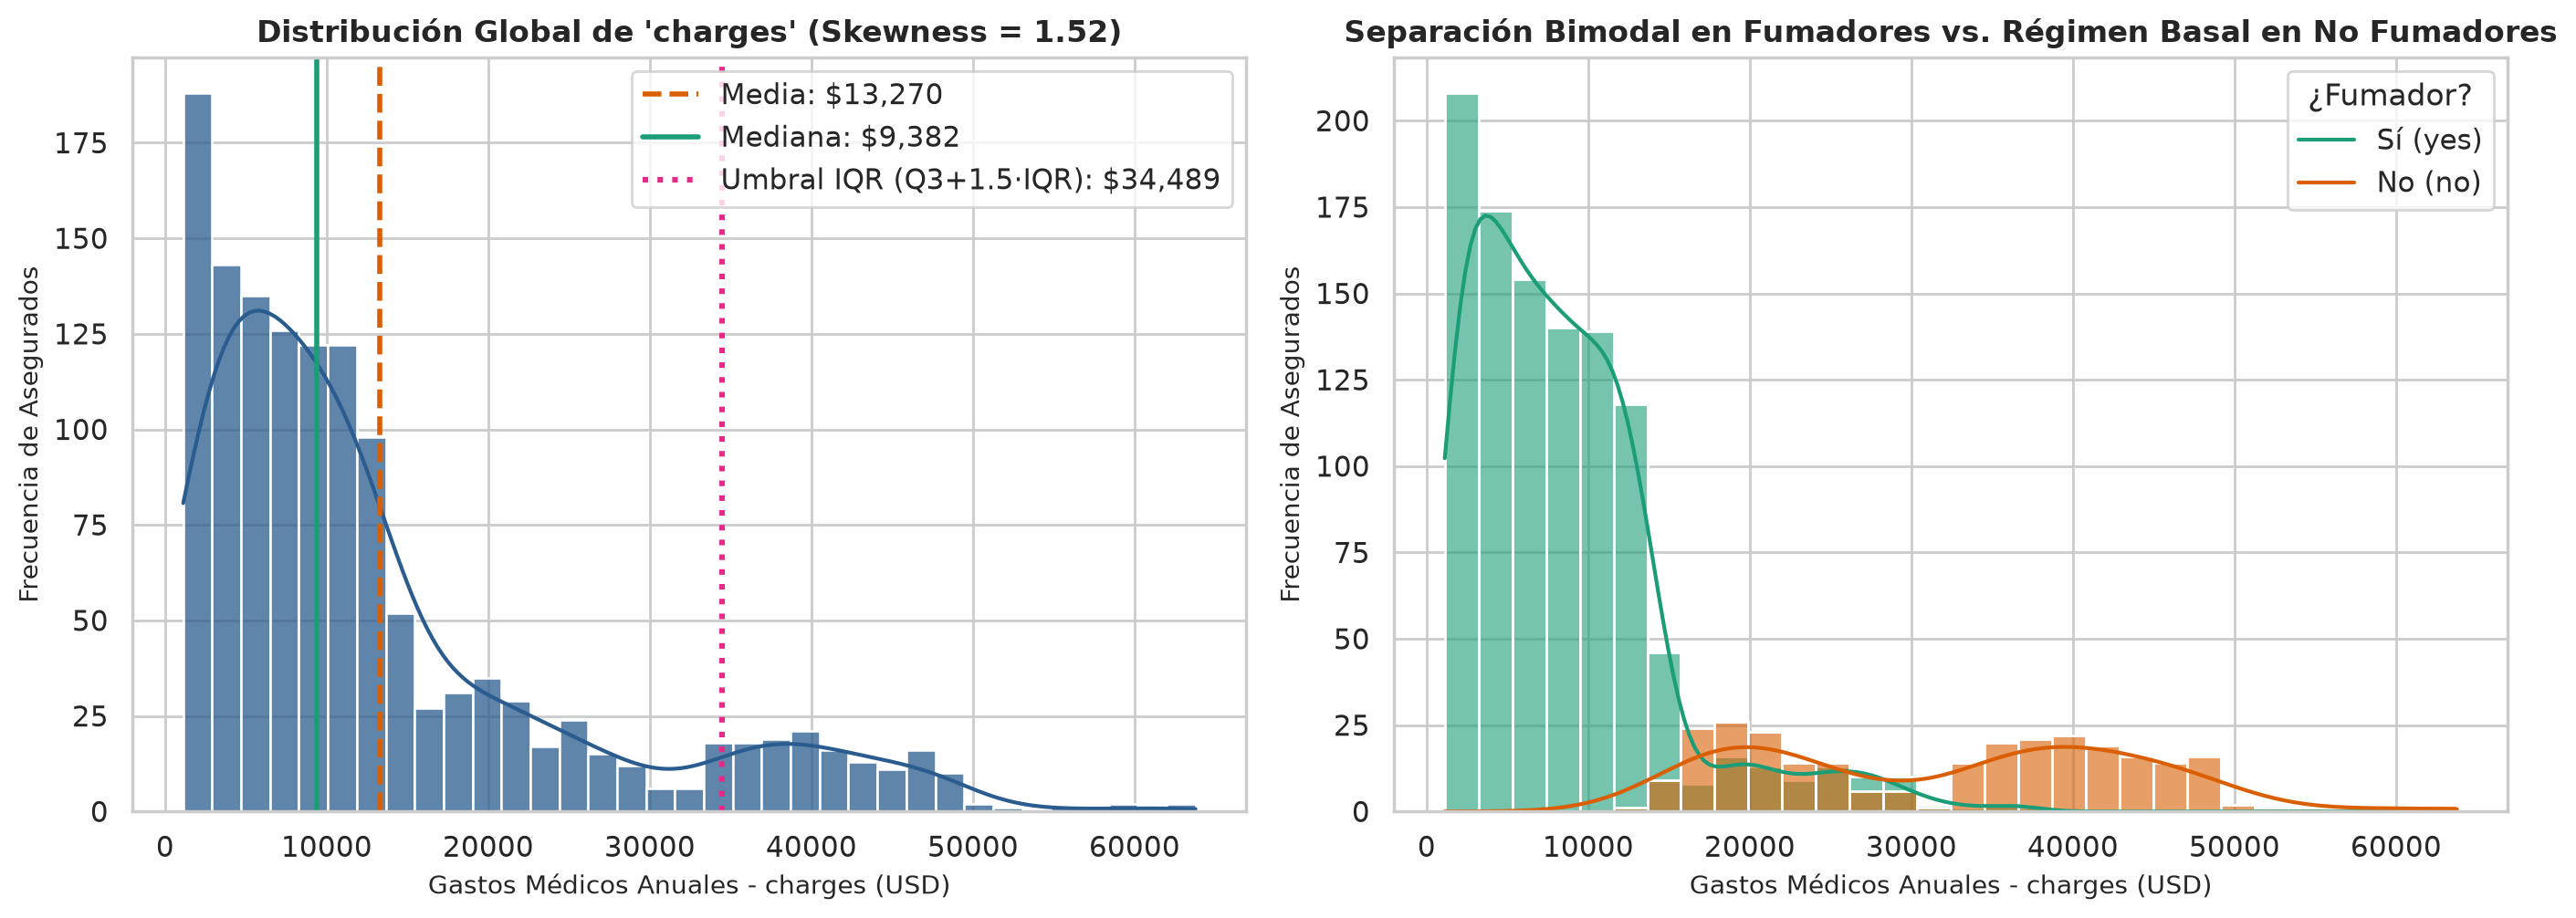
\includegraphics[width=0.92\textwidth]{images/eda_charges_distribution.png}
\caption{\textbf{Distribución de Gastos Médicos (\texttt{charges}).} Asimetría derecha ($\text{Skewness}=1.5159$) y bimodalidad al condicionar por tabaquismo.}
\end{figure}

\begin{figure}[H]
\centering
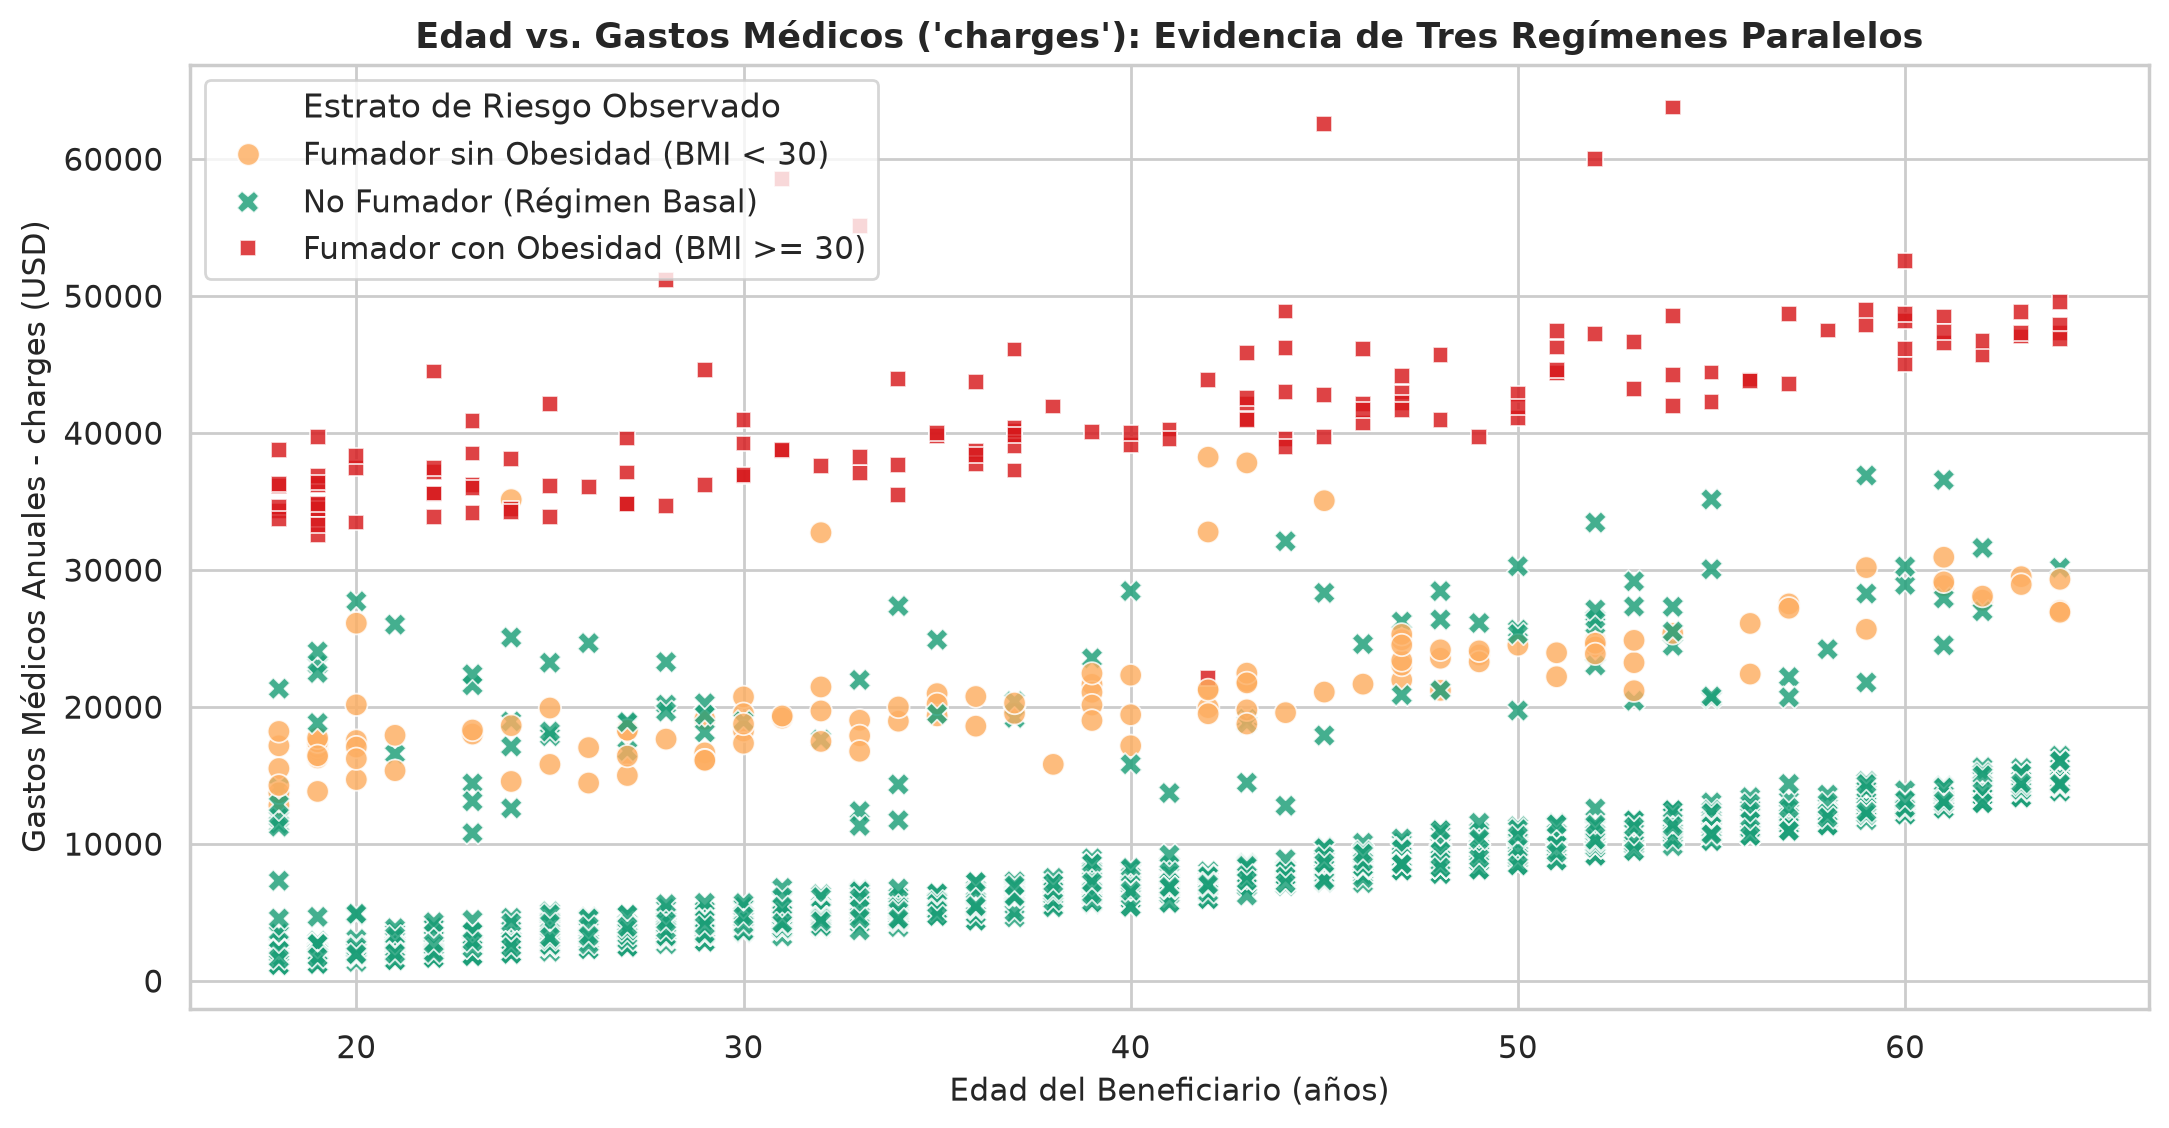
\includegraphics[width=0.88\textwidth]{images/eda_age_vs_charges.png}
\caption{\textbf{Edad vs. Cargos Médicos.} Evidencia visual de tres bandas paralelas según tabaquismo y obesidad.}
\end{figure}

\begin{figure}[H]
\centering
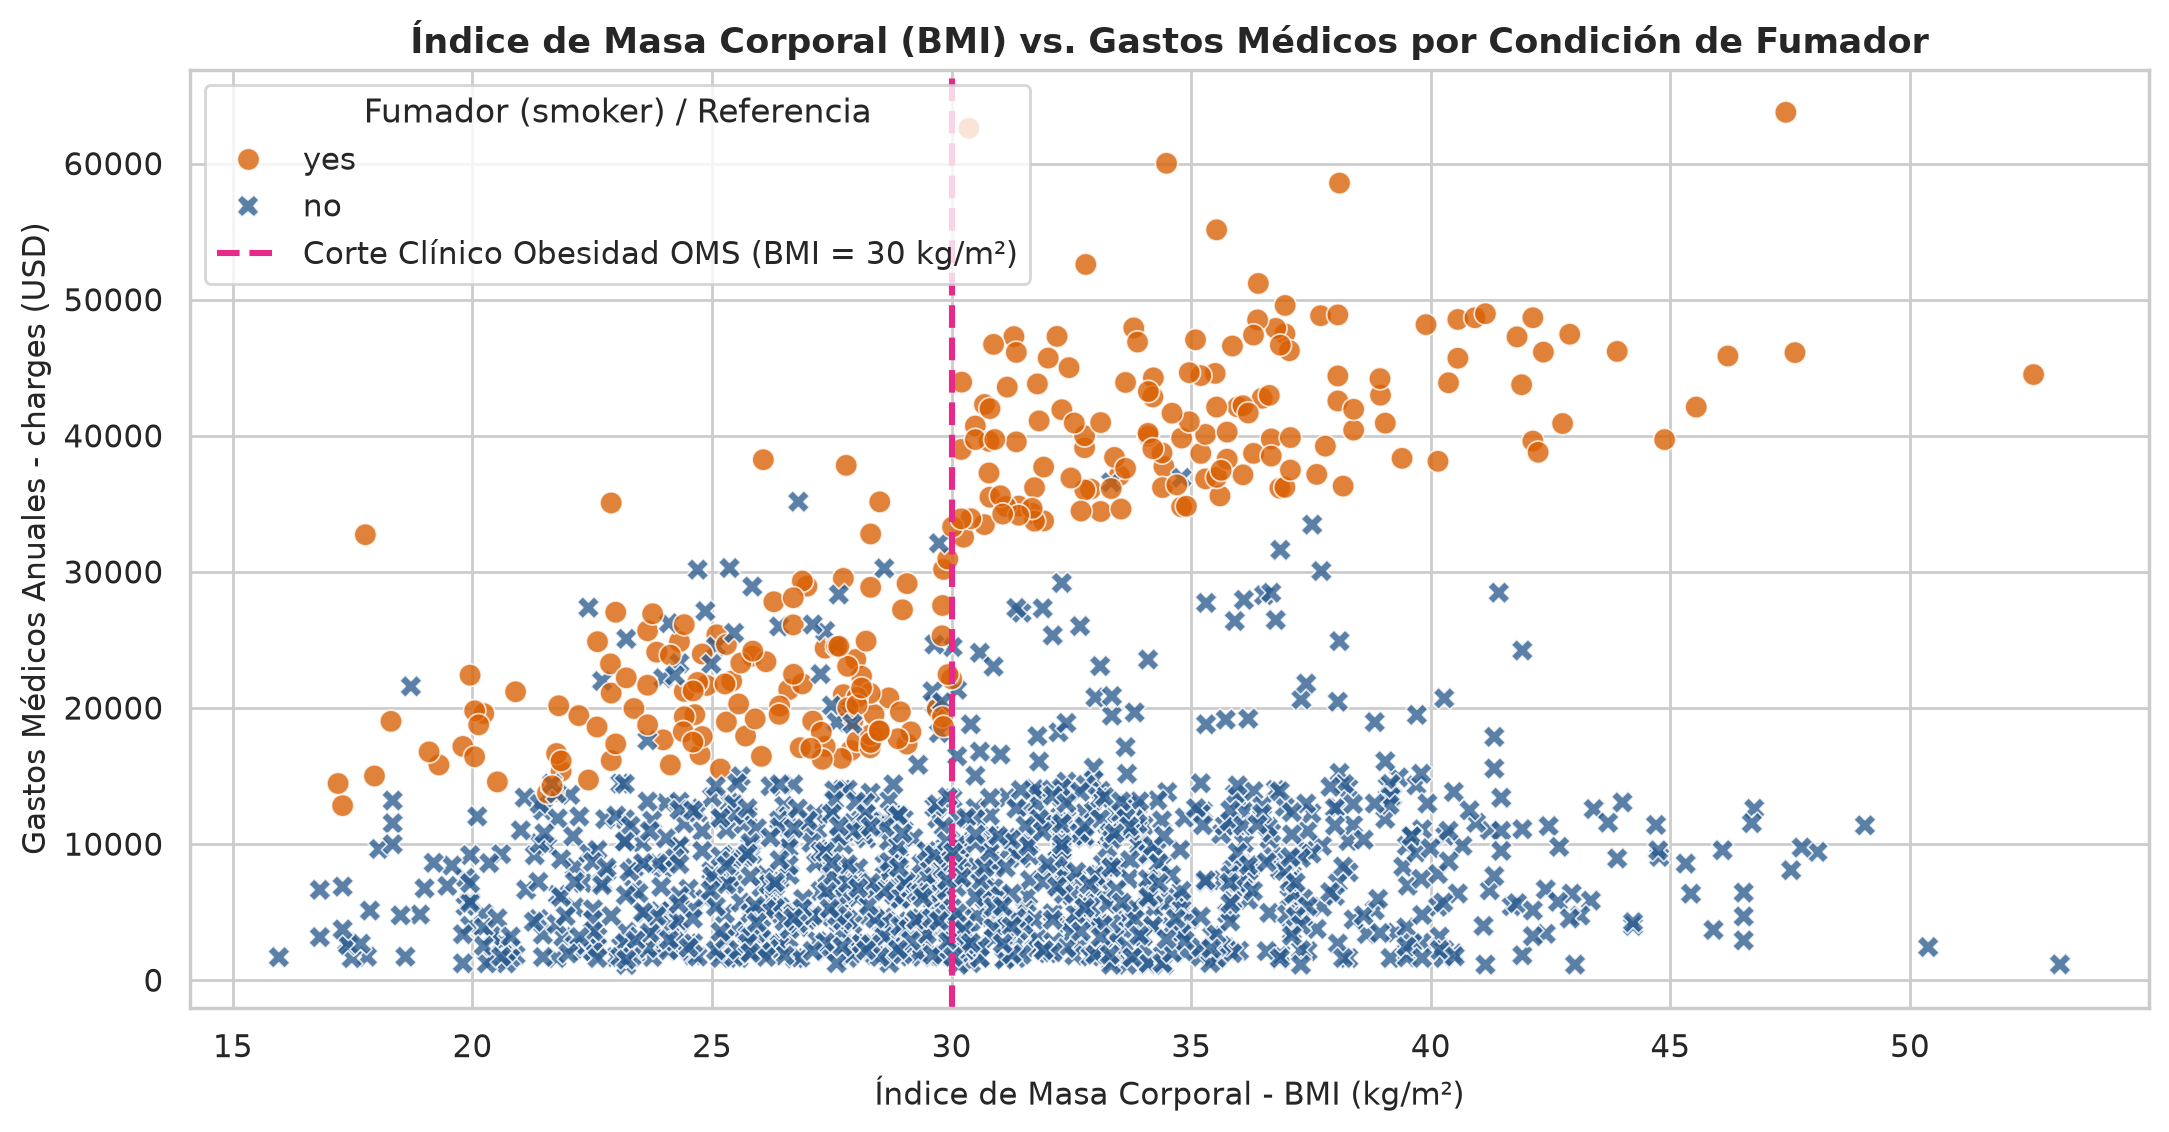
\includegraphics[width=0.88\textwidth]{images/eda_bmi_vs_charges.png}
\caption{\textbf{BMI vs. Cargos Médicos.} Salto no lineal a partir del umbral clínico de obesidad OMS ($BMI \ge 30\text{ kg/m}^2$).}
\end{figure}

\begin{figure}[H]
\centering
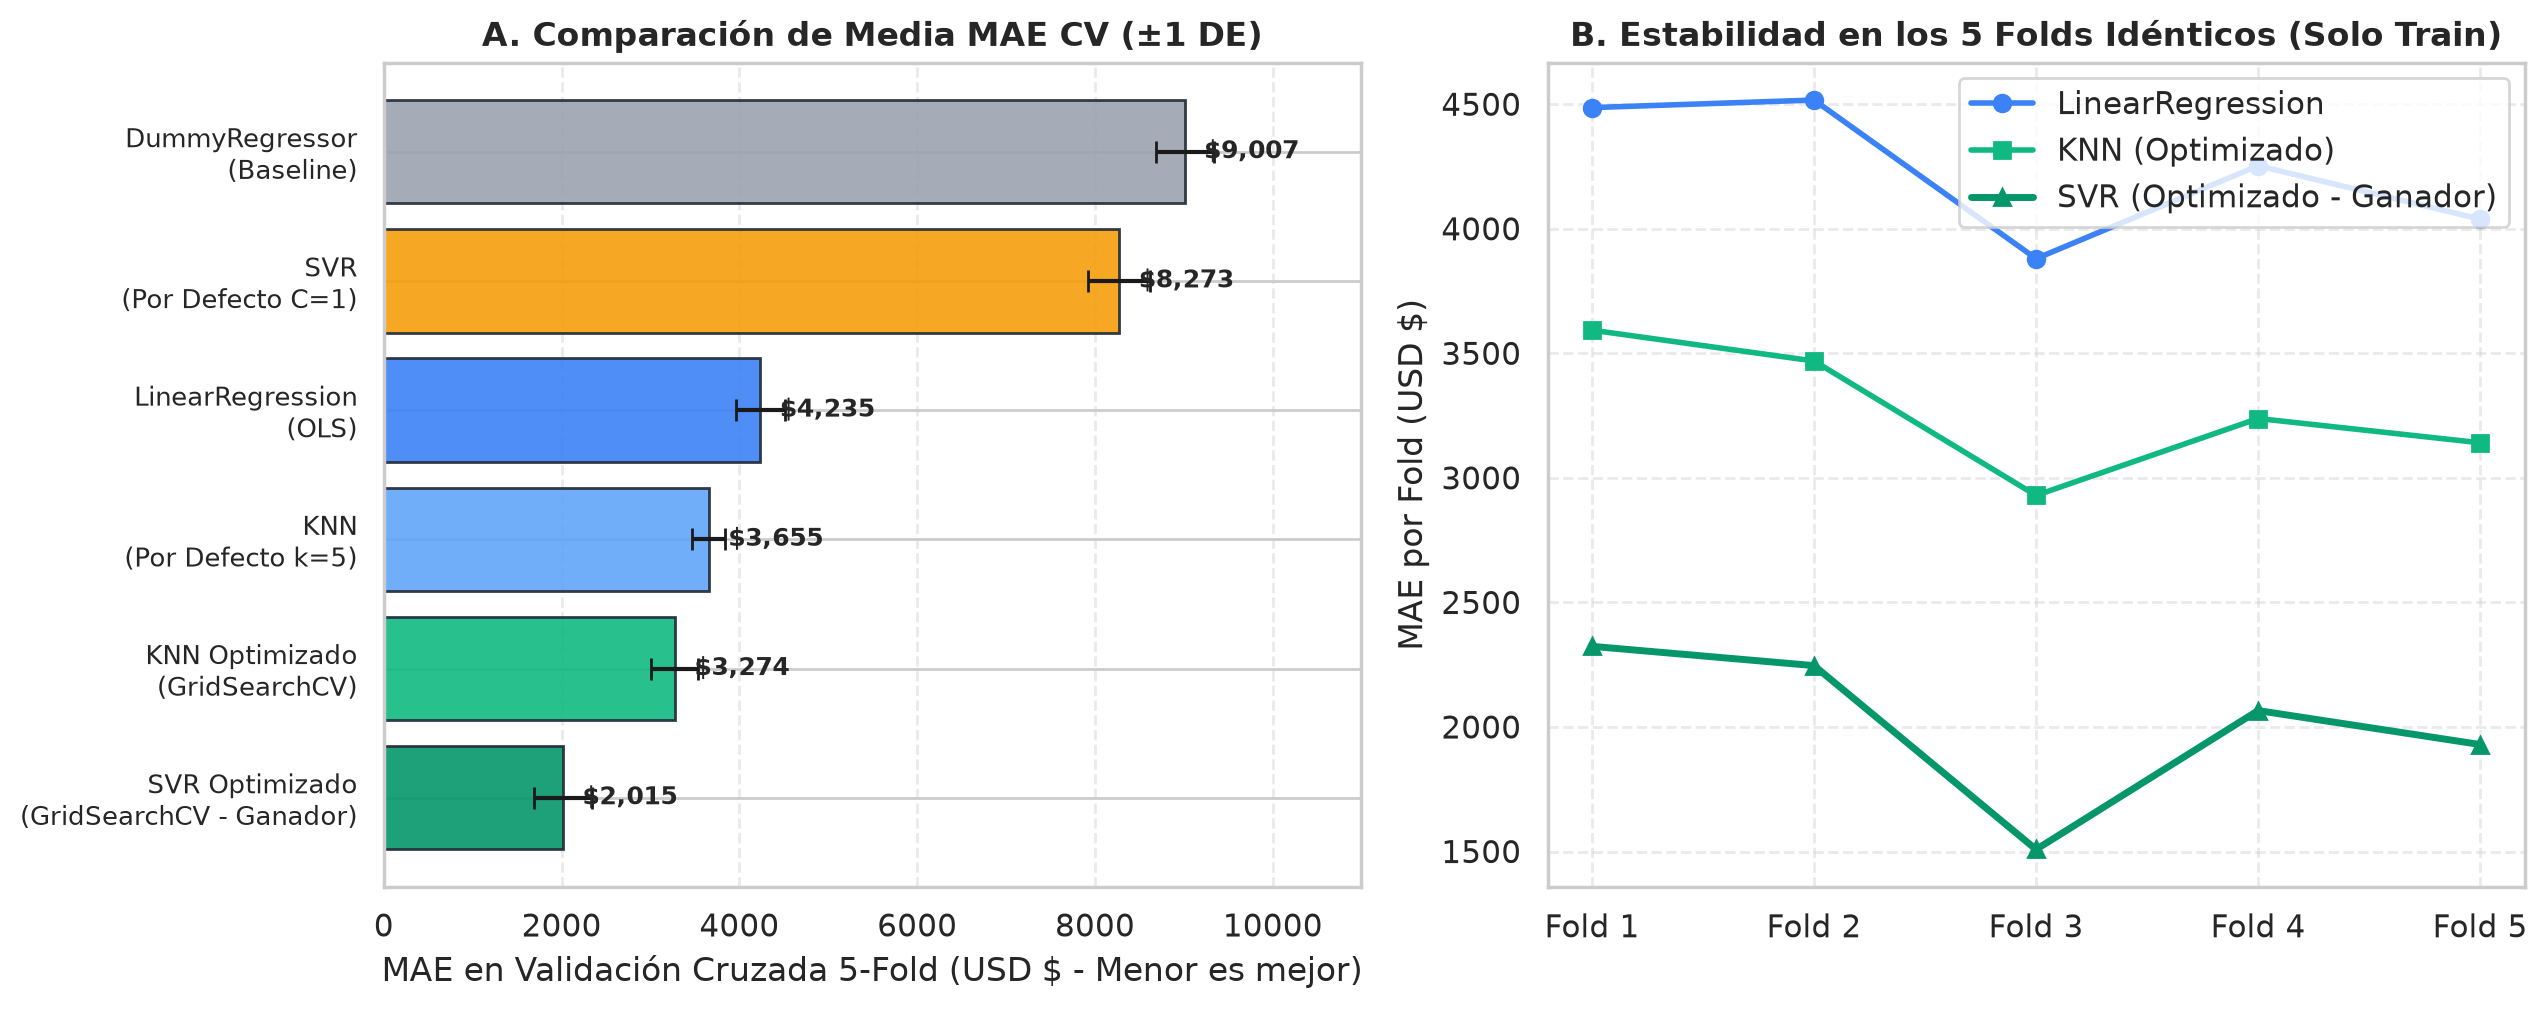
\includegraphics[width=0.88\textwidth]{images/ml_cv_comparison.png}
\caption{\textbf{Comparación en Validación Cruzada 5-Fold.} Reducción drástica del error de SVR tras GridSearchCV.}
\end{figure}

\begin{figure}[H]
\centering
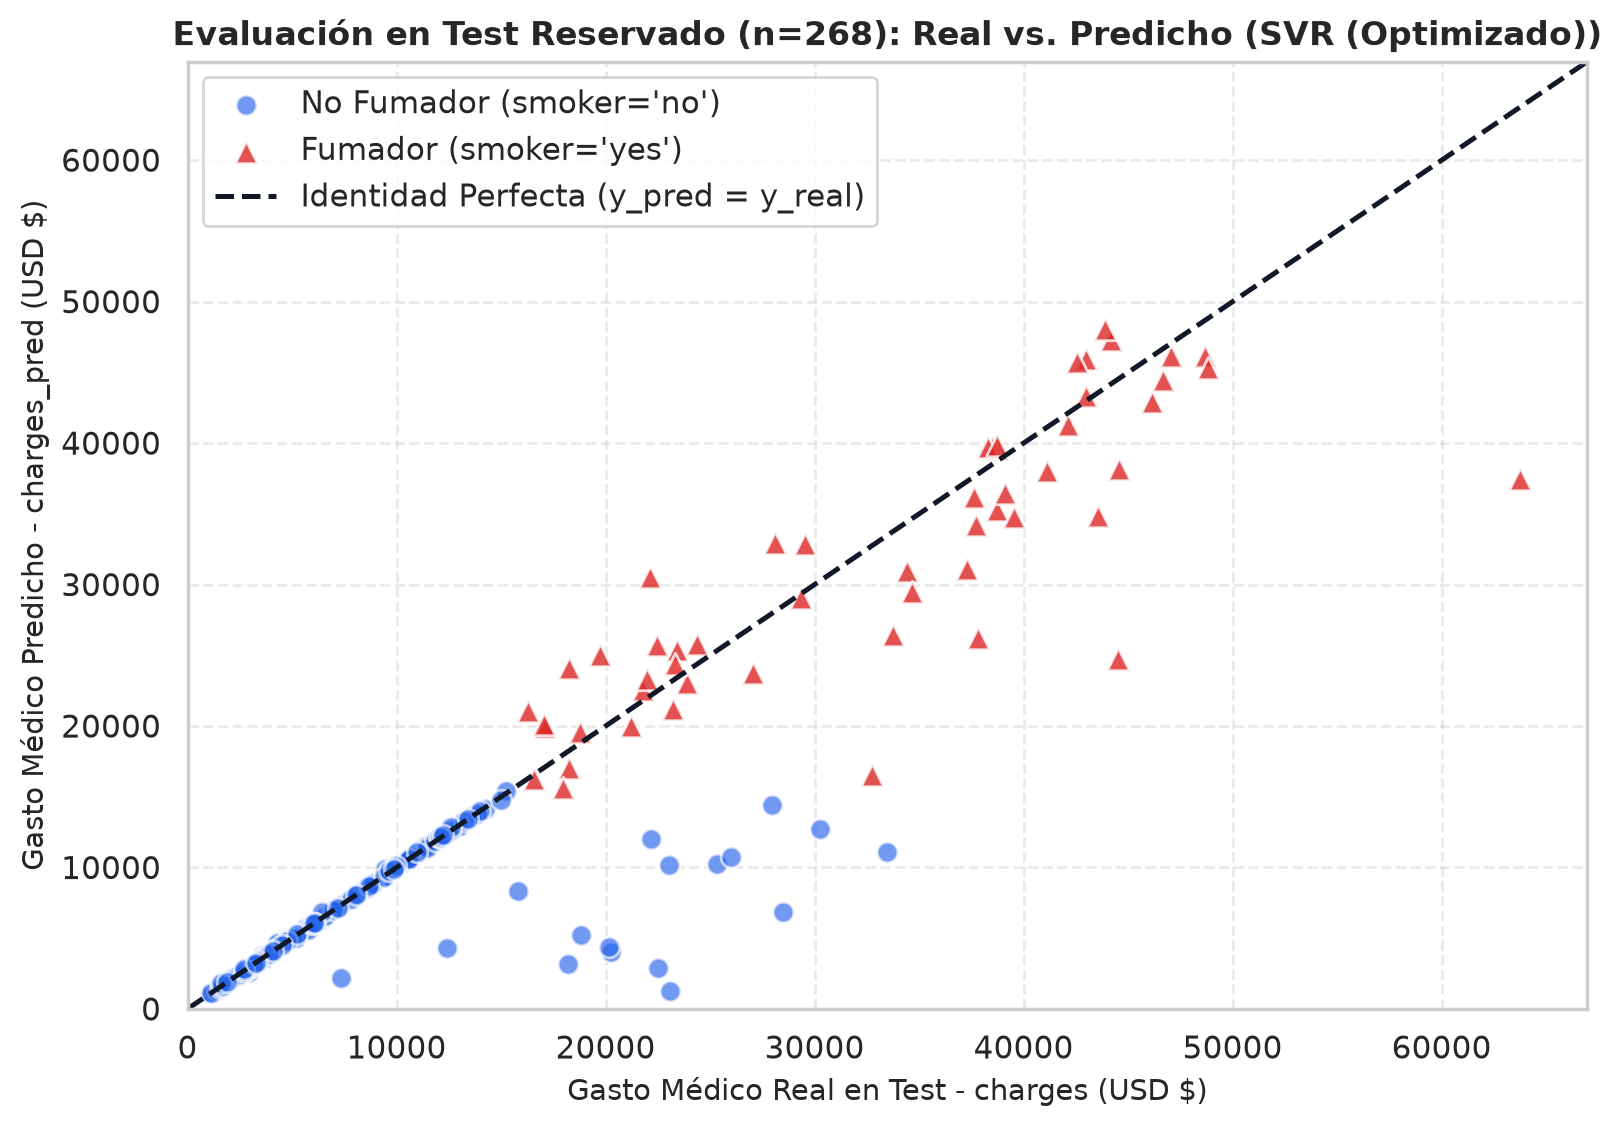
\includegraphics[width=0.82\textwidth]{images/ml_real_vs_pred.png}
\caption{\textbf{Valores Reales vs. Predichos en Conjunto Reservado ($n=268$).} Ajuste sobre la diagonal teórica de identidad.}
\end{figure}

\begin{figure}[H]
\centering
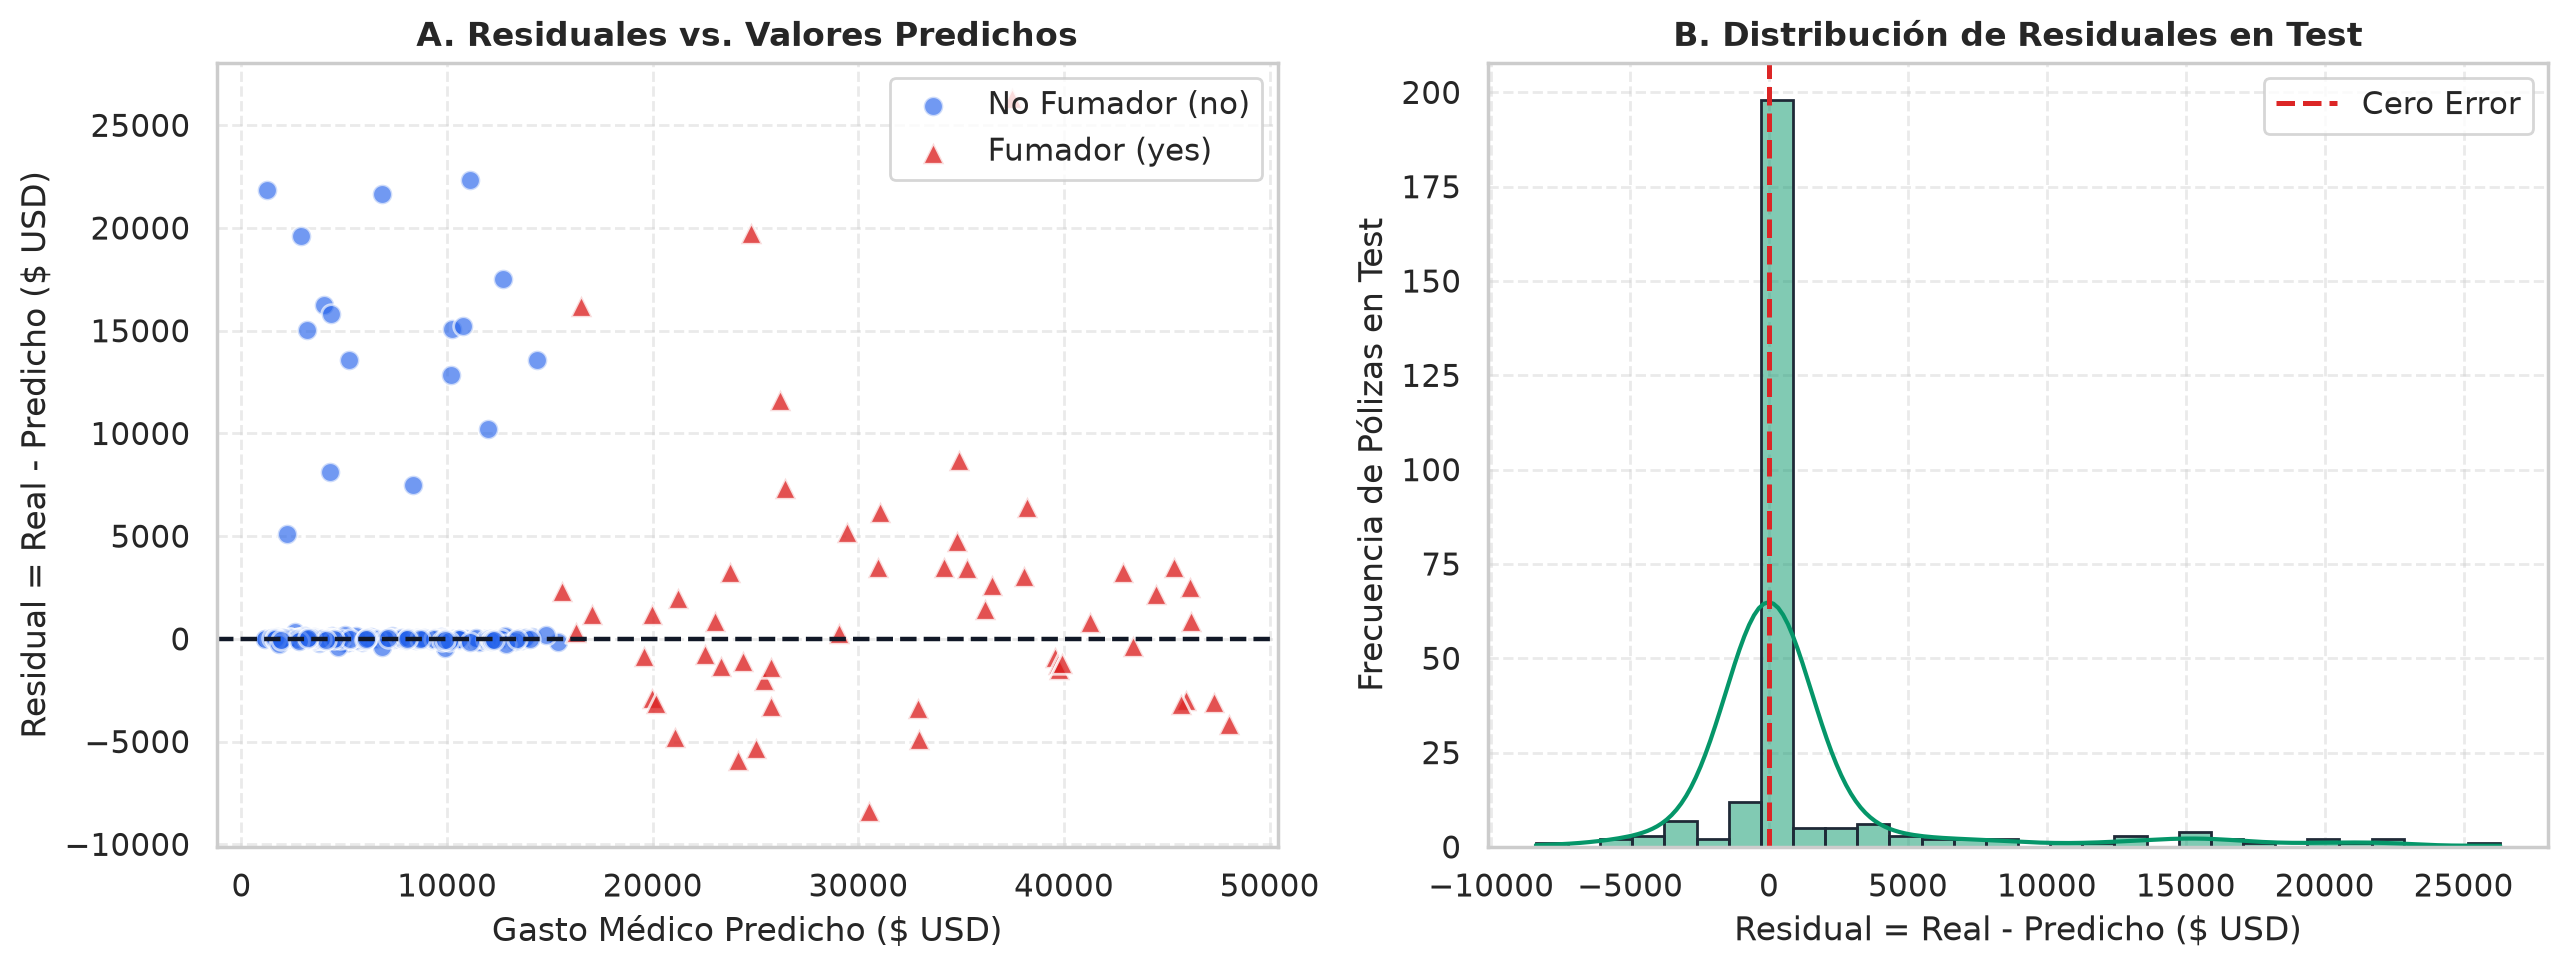
\includegraphics[width=0.88\textwidth]{images/ml_residuals_analysis.png}
\caption{\textbf{Diagnóstico de Residuales ($e_i = y_i - \hat{y}_i$).} Mediana de error absoluto de solo \$40.14 USD en test.}
\end{figure}

\begin{figure}[H]
\centering
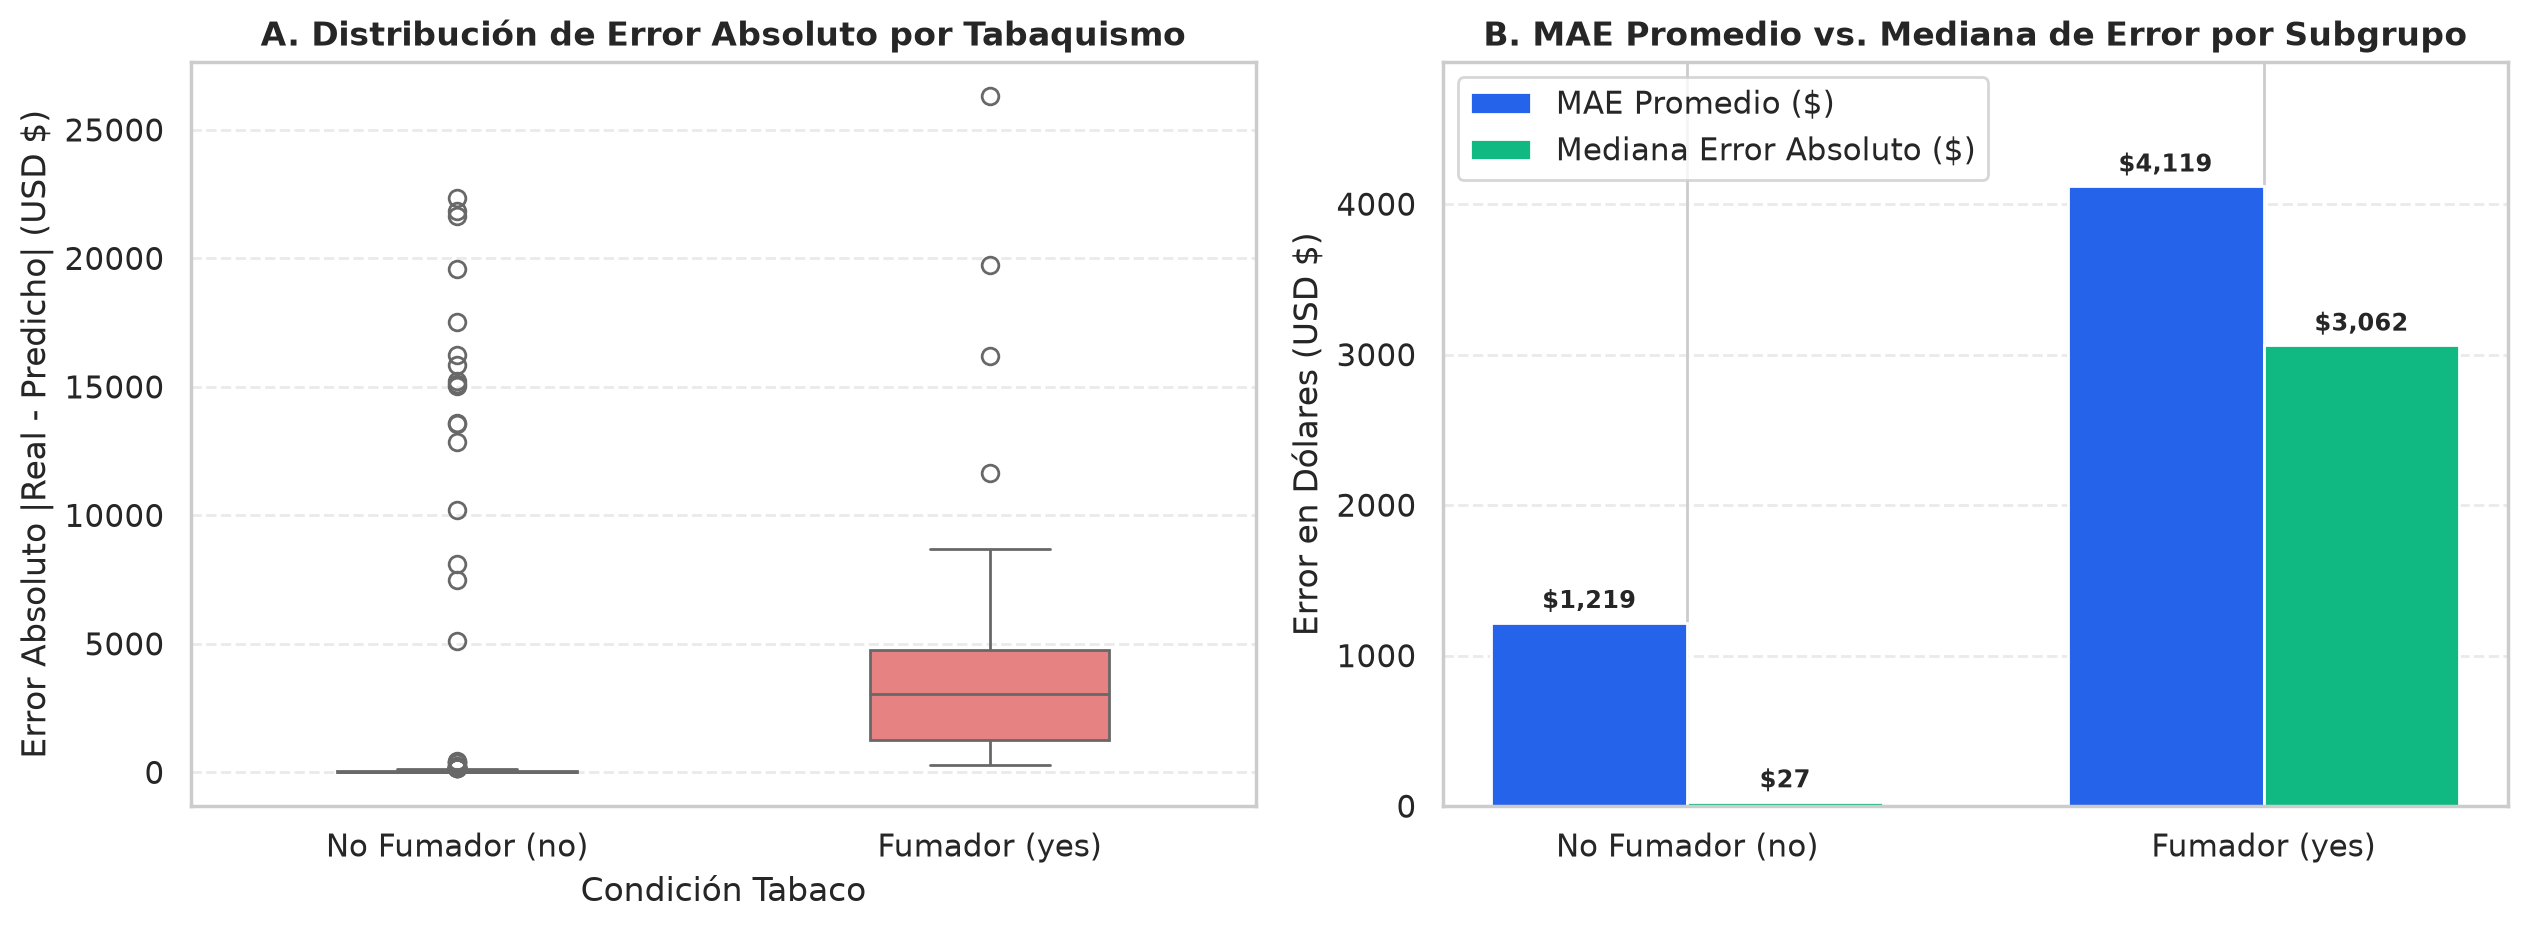
\includegraphics[width=0.88\textwidth]{images/ml_smoker_error_comparison.png}
\caption{\textbf{Análisis de Errores por Subgrupos de Tabaquismo.} Dispersión y medianas de error en fumadores y no fumadores.}
\end{figure}

\section{Discusión Crítica y Requisitos Específicos del Grupo 02}

\subsection{Requisito Específico: Comparativa MAE Fumadores vs. No Fumadores}
En cumplimiento estricto del encargo del Grupo 02, se analizó el comportamiento del modelo en el conjunto de prueba reservado ($n = 268$) desglosado por hábito de tabaquismo:

\begin{table}[H]
\centering
\caption{Desglose de Métricas en Test Reservado por Condición de Tabaquismo}
\footnotesize
\begin{tabularx}{\textwidth}{l c c c c c c c}
\toprule
\textbf{Subgrupo} & \textbf{Pólizas ($n$)} & \textbf{Proporción} & \textbf{Gasto Medio (\$)} & \textbf{MAE (\$)} & \textbf{Mediana Error (\$)} & \textbf{MAE Rel.} & \textbf{$R^2$ Intra} \\
\midrule
\textbf{No Fumadores (\texttt{'no'})} & 214 & 79.85\% & \$7,862.09 & \textbf{\$1,219.08} & \textbf{\$27.38} & 15.51\% & 0.4344 \\
\textbf{Fumadores (\texttt{'yes'})} & 54 & 20.15\% & \$33,204.10 & \textbf{\$4,119.27} & \textbf{\$3,061.69} & \textbf{12.41\%} & \textbf{0.6778} \\
\bottomrule
\end{tabularx}
\end{table}

\noindent\textbf{Interpretación Metodológica y Precaución No Causal:}
\begin{enumerate}[leftmargin=*]
    \item \textbf{Efecto de Escala Monetaria vs. Precisión Relativa:} El MAE nominal de fumadores ($\$4,119.27$) triplica al de no fumadores ($\$1,219.08$). No obstante, este fenómeno se debe a que los fumadores operan en una escala monetaria $4.2$ veces superior ($\$33,204$ vs. $\$7,862$). En términos relativos al gasto medio, el modelo comete menor error porcentual en fumadores ($12.41\%$) que en no fumadores ($15.51\%$), y su varianza explicada intra-grupo ($R^2 = 0.6778$) es sustancialmente superior.
    \item \textbf{Advertencia de No Causalidad:} La correlación entre \texttt{smoker = 'yes'} y cargos médicos elevados constituye una \textbf{asociación estadística observacional}. El diseño experimental no asignó tratamientos aleatorios ni midió variables confusoras esenciales (antecedentes laborales, carga genética, alimentación). Por tanto, \textbf{no debe inferirse causalidad médica directa} a partir de las ponderaciones del modelo.
\end{enumerate}

\subsection{Análisis por Niveles de Gasto Real}
\begin{itemize}[leftmargin=*]
    \item \textbf{Estrato Bajo ($< \$5,000$, $n=84$):} $\text{MAE} = \$47.76$ USD (Mediana: $\$25.82$). El modelo ajusta con precisión absoluta sobre asegurados jóvenes no fumadores.
    \item \textbf{Estrato Medio ($\$5,000 - \$15,000$, $n=114$):} $\text{MAE} = \$163.43$ USD (Mediana: $\$25.71$).
    \item \textbf{Estrato Alto ($> \$15,000$, $n=70$):} $\text{MAE} = \$6,581.14$ USD (Mediana: $\$3,402.86$). Concentra los mayores errores nominales debido a hospitalizaciones atípicas en no fumadores y dispersión de tratamientos oncológicos.
\end{itemize}

\section{Conclusiones, Recomendaciones y Dictamen de Despliegue}

\subsection{Cinco Conclusiones Respaldadas por Evidencia}
\begin{enumerate}[leftmargin=*]
    \item \textbf{Superación Holgada de Metas:} El pipeline \texttt{SVR (Optimizado)} superó holgadamente todos los criterios de éxito prefijados, logrando en prueba reservada un $\text{MAE} = \$1,803.44$ USD (meta: $< \$3,500$) y $R^2 = 0.8496$ (meta: $\ge 0.75$), con una reducción del $81.20\%$ del error respecto al baseline ingenuo.
    \item \textbf{Invalidez del Supuesto Lineal Puro:} La comparación demostró que la regresión lineal aditiva es insuficiente ($\text{MAE} = \$4,234.98$) para capturar la sinergia abrupta entre tabaquismo y obesidad ($BMI \ge 30$).
    \item \textbf{Transformación por Optimización:} \texttt{GridSearchCV} permitió pasar a SVR de un severo subajuste por parámetros por defecto ($\text{MAE} = \$8,272.97$, $C=1.0$) al liderazgo indiscutible ($\text{MAE} = \$2,014.67$, $C=10,000$), reduciendo el error en un $75.65\%$.
    \item \textbf{Resistencia ante Asimetría Extrema:} La formulación $\epsilon$-insensible de SVR neutralizó la influencia de los 139 valores atípicos ($10.39\%$), alcanzando una mediana de error absoluto de solo $\$40.14$ USD.
    \item \textbf{Blindaje Metodológico Anti-Fuga:} La partición 80/20 previa y el encapsulamiento en \texttt{ColumnTransformer} aseguraron cero fuga de datos (0 filas compartidas), garantizando reproducibilidad científica total.
\end{enumerate}

\subsection{Tres Mejoras Futuras Priorizadas}
\begin{enumerate}[leftmargin=*]
    \item \textbf{Prioridad 1:} Incorporación de historial de reclamos previos del año $t-1$ y biomarcadores clínicos (presión arterial, glucosa) para predecir hospitalizaciones no tabáquicas.
    \item \textbf{Prioridad 2:} Implementación de intervalos de predicción conformal al $90\%$ de confianza para el cálculo de reservas actuariales estocásticas.
    \item \textbf{Prioridad 3:} Evaluación de modelos de ensamble de gradiente (\texttt{LightGBM}) con restricciones de monotonicidad positiva respecto a la edad.
\end{enumerate}

\subsection{Dictamen Argumentado de Despliegue}
\textbf{APROBADO PARA DESPLIEGUE EN MODO PILOTO ACTUARIAL ASISTIDO (\textit{SHADOW TESTING})}. No se autoriza su aplicación para tarificación individual 100\% automatizada sin supervisión humana hasta incorporar reaseguro \textit{stop-loss} e indexación por inflación médica anual.

\section*{Referencias Bibliográficas (APA 7)}
\begin{enumerate}[leftmargin=*]
    \item Choi, M. (2018). \textit{Medical Cost Personal Datasets: Insurance Forecast by using Linear Regression}. Kaggle Datasets. \url{https://www.kaggle.com/datasets/mirichoi0218/insurance}
    \item Lantz, B. (2019). \textit{Machine Learning with R: Expert techniques for predictive modeling to solve problems in a dynamic world} (3.ª ed.). Packt Publishing.
    \item Pedregosa, F., et al. (2011). Scikit-learn: Machine Learning in Python. \textit{Journal of Machine Learning Research}, 12, 2825--2830.
    \item Smola, A. J., \& Schölkopf, B. (2004). A tutorial on support vector regression. \textit{Statistics and Computing}, 14(3), 199--222.
    \item World Health Organization. (2021). \textit{Obesity and overweight: Key facts}. WHO Media Centre.
\end{enumerate}

\end{document}
